\documentclass[manuscript,screen,review]{acmart}

\usepackage{graphicx}
\usepackage{booktabs}
\usepackage{listings}
\usepackage{xcolor}
\usepackage{amsmath}
\usepackage{subcaption}
\usepackage{url}
\usepackage{tikz}
\usetikzlibrary{arrows,positioning,fit,backgrounds,calc,shapes.misc}
\usepackage{array}
\newcolumntype{R}[1]{>{\raggedright\arraybackslash}p{#1}}

% Breakable monospace for file paths / identifiers in narrow table cells
\DeclareUrlCommand\fpath{\urlstyle{tt}}
\makeatletter\g@addto@macro\UrlBreaks{\do\_\do\.\do\-}\makeatother

\setcopyright{none}
\settopmatter{printacmref=false}
\renewcommand\footnotetextcopyrightpermission[1]{}
\acmConference[CSD 2026]{Computer System Design Course Project}{September 2026}{IIT Bhilai, India}
\acmYear{2026}

\lstset{
  basicstyle=\ttfamily\footnotesize,
  breaklines=true,
  frame=single,
  backgroundcolor=\color{gray!10},
  keywordstyle=\color{blue}\bfseries,
  commentstyle=\color{green!60!black},
  stringstyle=\color{red},
  columns=fullflexible
}

\begin{document}

\title{Bhagiratha: An AI-Enabled Geospatial System for Village Pond Site Selection and Catchment Delineation}

\author{Rahul Seera}
\affiliation{%
  \institution{Indian Institute of Technology Bhilai}
  \city{Durg}
  \state{Chhattisgarh}
  \country{India}
}
\email{rahulseera.r2@gmail.com}

\begin{abstract}
Village ponds (\textit{Amrit Sarovars}) are frequently excavated at locations chosen for administrative convenience rather than hydrology, and consequently either stay dry or breach during the monsoon. This paper presents \textbf{Bhagiratha}, a web-based geospatial decision-support system that automates pond site selection, upstream catchment delineation, runoff estimation and pond dimensioning. The system ingests either raster Digital Elevation Models (SRTM~30\,m via OpenTopography) or vector contour maps (KML/KMZ), interpolates contours onto a regular grid with SciPy's Delaunay-based linear interpolation, conditions the surface with Priority-Flood depression filling, and routes flow with the D8 algorithm on a latitude-corrected metric grid. The pond site is chosen as the interior cell of maximum flow accumulation. Ten years of daily precipitation from the Open-Meteo archive yield the June--September monsoon depth, from which seasonal runoff volume is estimated with the volumetric form of the Rational Method ($Q = C \cdot I \cdot A$, $C = 0.35$); the pond is sized to hold 70\% of that volume at a depth between 2.5\,m and 4.5\,m. The application is an asynchronous FastAPI modular monolith with a Leaflet.js front end, PostgreSQL/PostGIS persistence with an automatic file-based fallback, a rounded-grid response cache, and a watchdog supervisor for a shared campus container. On a real 1\,m contour survey from Chhattisgarh (1,355 contours), the system selects a site at $21.24171^\circ$N, $81.28692^\circ$E draining a $3.9116\,\text{km}^2$ catchment, estimates $1.71\times10^6\,\text{m}^3$ of monsoon runoff, and completes end-to-end in about 3\,s.
\end{abstract}

\begin{CCSXML}
<ccs2012>
<concept><concept_id>10010405.10010432.10010437</concept_id><concept_desc>Applied computing~Earth and atmospheric sciences</concept_desc><concept_significance>500</concept_significance></concept>
<concept><concept_id>10002951.10003227.10003236.10003237</concept_id><concept_desc>Information systems~Geographic information systems</concept_desc><concept_significance>300</concept_significance></concept>
</ccs2012>
\end{CCSXML}
\ccsdesc[500]{Applied computing~Earth and atmospheric sciences}
\ccsdesc[300]{Information systems~Geographic information systems}

\keywords{Hydrological Modeling, Catchment Delineation, D8 Flow Direction, Rational Method, Village Pond Planning, GIS, FastAPI, Leaflet.js}

\maketitle

% ======================================================================
\section{Introduction and Problem Statement}
\label{sec:intro}
Under national water-conservation programmes such as \textit{Mission Amrit Sarovar}, village administrators must choose where to excavate community ponds. Manual site selection suffers from three recurring problems:
\begin{enumerate}
    \item \textbf{Subjective siting:} ponds are placed on available land rather than on natural drainage lines, so little runoff reaches them.
    \item \textbf{Unknown catchment:} the upstream area that drains to a candidate site cannot be reliably delineated by hand over several square kilometres.
    \item \textbf{Hydraulic mismatch:} without linking catchment area to historical rainfall, ponds are either too small (overflow and embankment breach) or too large (never fill).
\end{enumerate}
Bhagiratha lets a non-expert user click a point, draw a candidate land parcel, or upload a contour map, and returns (1) a recommended pond location, (2) the delineated catchment boundary, (3) the expected monsoon runoff volume, (4) recommended depth, surface area and capacity, and (5) a 0--100 suitability score, all overlaid on satellite imagery.

% ======================================================================
\section{System Architecture}
\label{sec:arch}
Four quality attributes drive the architecture: \emph{correctness} of the hydrological result, \emph{interactive latency} (seconds, not minutes, per analysis), \emph{resilience} on a shared container with one CPU, no database service and partial internet access, and \emph{deployability} as a single process with no mandatory infrastructure. Following the HLD, Bhagiratha is an asynchronous \textbf{modular monolith}: one FastAPI process whose modules are separated by narrow, typed interfaces (Pydantic models in, Pydantic models out), so each engine can be tested, replaced or moved to its own service without touching the others.

Figure~\ref{fig:arch} shows the resulting layers.
\begin{itemize}
    \item The \textbf{presentation layer} is a single-page Leaflet application. It holds no domain logic: it renders whatever the API returns, including the \texttt{warnings} array.
    \item The \textbf{API layer} validates every request against a schema, consults the response cache, and orchestrates the engines. I/O-bound calls run as concurrent \texttt{asyncio} tasks, and CPU-bound work is moved to worker threads.
    \item Four \textbf{domain engines} carry the logic. The terrain engine turns a DEM or contour map into a pond site and catchment; the precipitation engine turns a location into a 10-year monsoon rainfall depth; the recommendation engine combines them into runoff, dimensions and a score; village search resolves place names.
    \item The \textbf{persistence layer} is chosen at startup: PostGIS when reachable, otherwise JSON files. Bundled reference data and temporary rasters live beside it.
    \item An \textbf{operations} layer of two shell scripts supervises the process.
\end{itemize}

% ---------- Figure: layered component architecture ----------
\begin{figure*}[t]
\centering
\resizebox{\linewidth}{!}{%
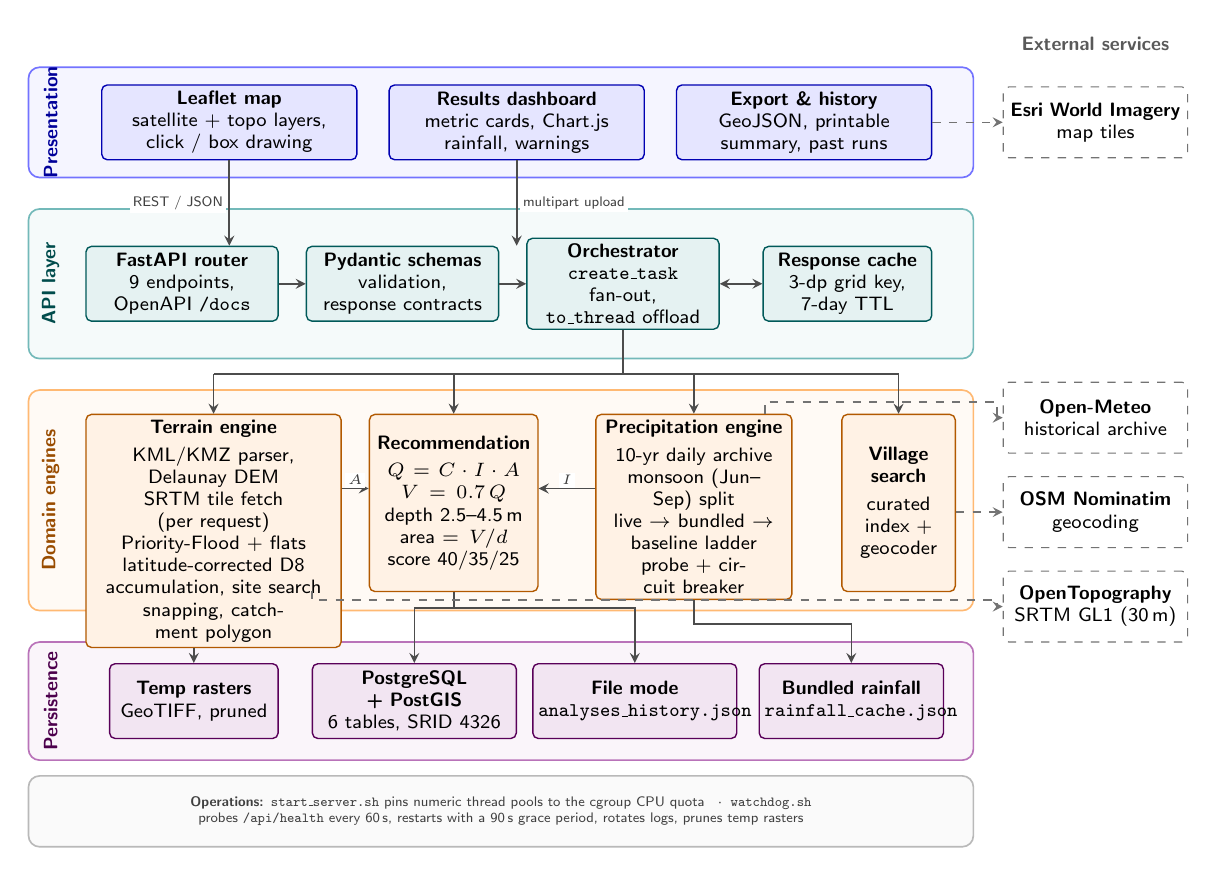
\begin{tikzpicture}[
  font=\sffamily\scriptsize,
  >=stealth,
  comp/.style={draw=#1!70!black, fill=#1!10, rounded corners=2pt, align=center, minimum height=0.95cm, inner sep=2pt, line width=0.5pt},
  comp/.default=gray,
  band/.style={draw=#1!55, fill=#1!4, rounded corners=4pt, line width=0.6pt},
  bandlabel/.style={rotate=90, font=\sffamily\scriptsize\bfseries, text=#1!60!black, anchor=center},
  ext/.style={draw=black!55, fill=white, rounded corners=2pt, align=center, minimum height=0.9cm, text width=2.2cm, inner sep=2pt, dashed},
  flow/.style={->, line width=0.6pt, draw=black!70},
  net/.style={->, line width=0.6pt, draw=black!55, dashed},
  lbl/.style={font=\sffamily\tiny, fill=white, inner sep=1pt, text=black!75},
]
\def\bw{12.0}
% ---- bands ----
\draw[band=blue]   (0,8.35) rectangle (\bw,9.75);
\draw[band=teal]   (0,6.05) rectangle (\bw,7.95);
\draw[band=orange] (0,2.85) rectangle (\bw,5.65);
\draw[band=violet] (0,0.95) rectangle (\bw,2.45);
\draw[band=gray]   (0,-0.15)  rectangle (\bw,0.75);
\node[bandlabel=blue]   at (0.28,9.05) {Presentation};
\node[bandlabel=teal]   at (0.28,7.0)  {API layer};
\node[bandlabel=orange] at (0.28,4.25) {Domain engines};
\node[bandlabel=violet] at (0.28,1.7)  {Persistence};

% ---- presentation ----
\node[comp=blue, text width=3.1cm] (map)  at (2.55,9.05) {\textbf{Leaflet map}\\satellite + topo layers,\\click / box drawing};
\node[comp=blue, text width=3.1cm] (dash) at (6.2,9.05)  {\textbf{Results dashboard}\\metric cards, Chart.js\\rainfall, warnings};
\node[comp=blue, text width=3.1cm] (exp)  at (9.85,9.05) {\textbf{Export \& history}\\GeoJSON, printable\\summary, past runs};

% ---- API ----
\node[comp=teal, text width=2.3cm] (router) at (1.95,7.0) {\textbf{FastAPI router}\\9 endpoints,\\OpenAPI \texttt{/docs}};
\node[comp=teal, text width=2.3cm] (schema) at (4.75,7.0)  {\textbf{Pydantic schemas}\\validation,\\response contracts};
\node[comp=teal, text width=2.3cm] (orch)   at (7.55,7.0) {\textbf{Orchestrator}\\\texttt{create\_task} fan-out,\\\texttt{to\_thread} offload};
\node[comp=teal, text width=2.0cm] (cache)  at (10.4,7.0) {\textbf{Response cache}\\3-dp grid key,\\7-day TTL};

% ---- domain engines: Terrain -> Recommendation <- Precipitation ----
\node[comp=orange, text width=3.1cm, minimum height=2.25cm, anchor=north] (terrain) at (2.35,5.35) {\textbf{Terrain engine}\\[2pt]
  KML/KMZ parser, Delaunay DEM\\SRTM tile fetch (per request)\\Priority-Flood + flats\\latitude-corrected D8\\accumulation, site search\\snapping, catchment polygon};
\node[comp=orange, text width=2.0cm, minimum height=2.25cm, anchor=north] (rec) at (5.4,5.35) {\textbf{Recommendation}\\[2pt]
  $Q = C\cdot I\cdot A$\\$V = 0.7\,Q$\\depth 2.5--4.5\,m\\area $= V/d$\\score 40/35/25};
\node[comp=orange, text width=2.35cm, minimum height=2.25cm, anchor=north] (rain) at (8.45,5.35) {\textbf{Precipitation engine}\\[2pt]
  10-yr daily archive\\monsoon (Jun--Sep) split\\live $\to$ bundled $\to$\\baseline ladder\\probe + circuit breaker};
\node[comp=orange, text width=1.3cm, minimum height=2.25cm, anchor=north] (vil) at (11.05,5.35) {\textbf{Village search}\\[2pt]curated\\index +\\geocoder};

% ---- persistence ----
\node[comp=violet, text width=2.0cm] (tmp)  at (2.1,1.7)  {\textbf{Temp rasters}\\GeoTIFF, pruned};
\node[comp=violet, text width=2.45cm] (pg)  at (4.9,1.7) {\textbf{PostgreSQL + PostGIS}\\6 tables, SRID 4326};
\node[comp=violet, text width=2.45cm] (json) at (7.7,1.7) {\textbf{File mode}\\\texttt{analyses\_history.json}};
\node[comp=violet, text width=2.2cm] (rc)   at (10.45,1.7) {\textbf{Bundled rainfall}\\\texttt{rainfall\_cache.json}};

% ---- ops strip ----
\node[font=\sffamily\tiny, text=black!75, align=center, text width=11.4cm] at (\bw/2,0.3) {\textbf{Operations:} \texttt{start\_server.sh} pins numeric thread pools to the cgroup CPU quota \enspace$\cdot$\enspace \texttt{watchdog.sh} probes \texttt{/api/health} every 60\,s, restarts with a 90\,s grace period, rotates logs, prunes temp rasters};

% ---- external services ----
\node[font=\sffamily\scriptsize\bfseries, text=black!65] at (13.55,10.05) {External services};
\node[ext] (esri)   at (13.55,9.05) {\textbf{Esri World Imagery}\\map tiles};
\node[ext] (ometeo) at (13.55,5.3)  {\textbf{Open-Meteo}\\historical archive};
\node[ext] (nomi)   at (13.55,4.1)  {\textbf{OSM Nominatim}\\geocoding};
\node[ext] (otopo)  at (13.55,2.9)  {\textbf{OpenTopography}\\SRTM GL1 (30\,m)};

% ---- flows: presentation -> API ----
\draw[flow] (map.south) -- node[lbl, left, xshift=-1pt] {REST / JSON} (map.south |- router.north);
\draw[flow] (dash.south) -- node[lbl, right, xshift=1pt] {multipart upload} (dash.south |- schema.north);
\draw[net] (exp.east) -- (esri.west);
% ---- API internals ----
\draw[flow] (router) -- (schema);
\draw[flow] (schema) -- (orch);
\draw[flow, <->] (orch) -- (cache);
% ---- fan-out to engines ----
\coordinate (bus) at (0,5.85);
\draw[line width=0.6pt, draw=black!70] (orch.south) -- (orch.south |- bus);
\draw[line width=0.6pt, draw=black!70] (terrain.north |- bus) -- (vil.north |- bus);
\foreach \n in {terrain, rec, rain, vil} \draw[flow] (\n.north |- bus) -- (\n.north);
% ---- engine data flow ----
\draw[flow] (terrain.east |- 0,4.4) -- node[lbl, above] {$A$} (rec.west |- 0,4.4);
\draw[flow] (rain.west |- 0,4.4) -- node[lbl, above] {$I$} (rec.east |- 0,4.4);
% ---- persistence ----
\draw[flow] (terrain.south -| tmp.north) -- (tmp.north);
\draw[flow] (rec.south) -- ++(0,-0.2) -| (pg.north);
\draw[flow] (rec.south) -- ++(0,-0.2) -| (json.north);
\draw[flow] (rain.south) -- ++(0,-0.3) -| (rc.north);
% ---- network calls ----
\draw[net] (3.6,3.1) -- (3.6,2.98) -- (12.3,2.98) |- (otopo.west);
\draw[net] (9.35,5.35) -- (9.35,5.5) -- (12.3,5.5) |- (ometeo.west);
\draw[net] (vil.east |- nomi.west) -- (nomi.west);
\end{tikzpicture}}
\Description{Layered architecture. The browser presentation layer (Leaflet map, results dashboard, export and history) sends REST requests to the API layer (FastAPI router, Pydantic schemas, orchestrator, response cache). The orchestrator fans out to the domain engines: terrain, recommendation, precipitation and village search; terrain supplies area and slope and precipitation supplies rainfall depth to the recommendation engine. Terrain calls OpenTopography, precipitation calls Open-Meteo, village search calls Nominatim, and the map loads Esri tiles. Results persist in PostGIS or, without a database, in JSON files. An operations strip shows the start script and watchdog.}
\caption{Layered component architecture. $A$: catchment area and slope; $I$: monsoon rainfall depth. Solid arrows are in-process calls; dashed arrows are network calls to external services, each backed by a local fallback (\S\ref{sec:degrade}).}
\label{fig:arch}
\end{figure*}


\subsection{Request Lifecycle}
Figure~\ref{fig:pipeline} traces a contour-map request, the most complex path. The multipart upload is validated by type and size, then parsed and interpolated to a grid in a worker thread (about 1\,s together). The terrain engine conditions the grid, routes flow on a metric D8 grid, selects the pond cell and delineates its catchment in 0.16\,s. Only then is the rainfall query issued, because it needs the pond coordinates. Its result, with the catchment area and slope, feeds the recommendation engine, and the response returns both the numbers and the GeoJSON polygon.

Point and land-area requests replace parsing and interpolation with an SRTM download (about 12\,s, the dominant cost). In point mode the site is known up front, so the DEM download and rainfall query are started together and the rainfall latency disappears behind the download. A repeated point request is answered from the rounded-grid cache in milliseconds.

% ---------- Figure: analysis pipeline ----------
\begin{figure*}[t]
\centering
\resizebox{\linewidth}{!}{%
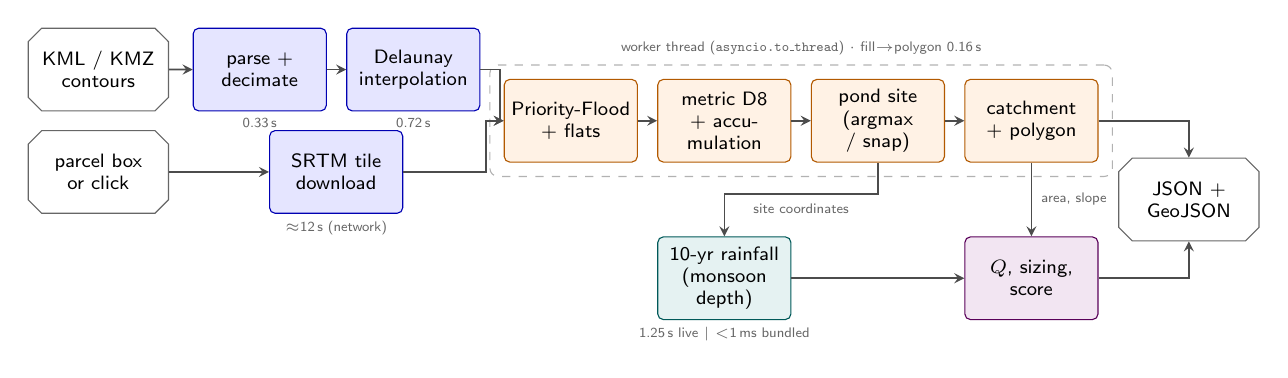
\begin{tikzpicture}[
  font=\sffamily\scriptsize, >=stealth,
  st/.style={draw=#1!70!black, fill=#1!10, rounded corners=2pt, align=center, text width=1.55cm, minimum height=1.05cm, inner sep=2pt},
  st/.default=orange,
  io/.style={draw=black!60, fill=white, align=center, text width=1.5cm, minimum height=1.05cm, inner sep=2pt, chamfered rectangle, chamfered rectangle xsep=2pt},
  flow/.style={->, line width=0.6pt, draw=black!70},
  t/.style={font=\sffamily\tiny, text=black!60},
]
\node[io] (kml) at (0,2.2) {KML / KMZ\\contours};
\node[io] (bbox) at (0,0.9) {parcel box\\or click};
\node[st=blue] (parse) at (2.05,2.2) {parse +\\decimate};
\node[t, below=-1pt of parse] {0.33\,s};
\node[st=blue] (grid) at (4.0,2.2) {Delaunay\\interpolation};
\node[t, below=-1pt of grid] {0.72\,s};
\node[st=blue] (srtm) at (3.02,0.9) {SRTM tile\\download};
\node[t, below=-1pt of srtm] {$\approx$12\,s (network)};
\node[st] (fill) at (6.0,1.55) {Priority-Flood\\+ flats};
\node[st] (d8) at (7.95,1.55) {metric D8\\+ accumulation};
\node[st] (site) at (9.9,1.55) {pond site\\(argmax / snap)};
\node[st] (catch) at (11.85,1.55) {catchment\\+ polygon};
\node[st=teal] (rain) at (7.95,-0.45) {10-yr rainfall\\(monsoon depth)};
\node[t, below=-1pt of rain] {1.25\,s live $\mid$ $<$1\,ms bundled};
\node[st=violet] (rec) at (11.85,-0.45) {$Q$, sizing,\\score};
\node[io] (out) at (13.85,0.55) {JSON +\\GeoJSON};
\draw[flow] (kml) -- (parse); \draw[flow] (parse) -- (grid);
\draw[flow] (bbox) -- (srtm);
\draw[flow] (grid.east) -- ++(0.25,0) |- (fill.west);
\draw[flow] (srtm.east) -- ++(1.05,0) |- (fill.west);
\draw[flow] (fill) -- (d8); \draw[flow] (d8) -- (site); \draw[flow] (site) -- (catch);
\draw[flow] (site.south) -- ++(0,-0.4) -| node[t, pos=0.25, below] {site coordinates} (rain.north);
\draw[flow] (rain) -- (rec);
\draw[flow] (catch) -- node[t, right] {area, slope} (rec);
\draw[flow] (catch.east) -| (out.north);
\draw[flow] (rec.east) -| (out.south);
\begin{scope}[on background layer]
\node[draw=black!30, dashed, rounded corners=3pt, fit=(fill)(catch)(d8), inner sep=5pt, label={[t]above:worker thread (\texttt{asyncio.to\_thread}) $\cdot$ fill$\to$polygon 0.16\,s}] {};
\end{scope}
\end{tikzpicture}}
\Description{Pipeline: contour files are parsed and interpolated, or an SRTM tile is downloaded for a parcel or click; the elevation grid is conditioned with Priority-Flood, routed with metric D8, the pond site is chosen, and the catchment is delineated. Rainfall for the site is looked up, then runoff, sizing and score are computed and returned as JSON and GeoJSON. Stage timings are annotated.}
\caption{Analysis pipeline with measured stage latencies (reference survey, development machine). Flow routing runs in a worker thread; where Open-Meteo is unreachable, rainfall comes from the bundled archive.}
\label{fig:pipeline}
\end{figure*}


\subsection{Deployment View}
Figure~\ref{fig:deploy} shows the production deployment. The container exposes port 3000 through host port 3247. \texttt{uvicorn} runs the application in file mode, and a shell loop runs the watchdog every 60\,s. Three properties of this environment, all discovered by measurement rather than assumed, shaped the design (\S\ref{sec:deploy}): the cgroup grants one CPU while the OS reports 120 cores; Open-Meteo and Nominatim are blocked while OpenTopography is reachable; and the disk is 99\% full.

% ---------- Figure: deployment ----------
\begin{figure}[t]
\centering
\resizebox{\linewidth}{!}{%
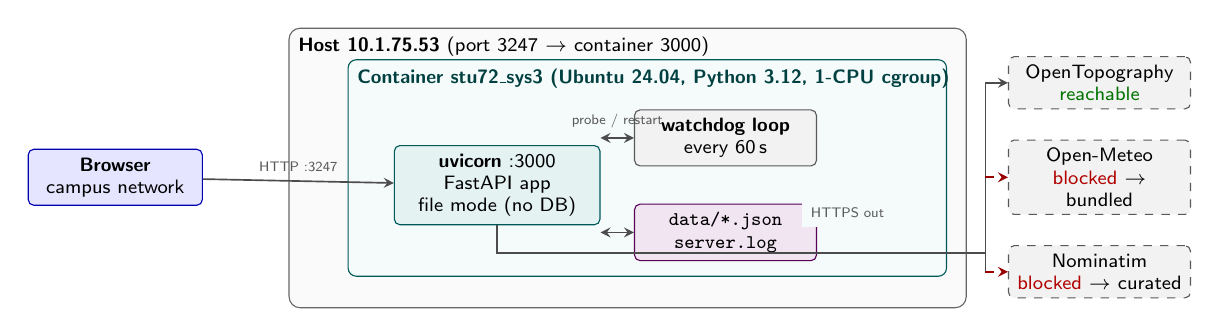
\begin{tikzpicture}[
  font=\sffamily\scriptsize, >=stealth,
  box/.style={draw=#1!70!black, fill=#1!10, rounded corners=2pt, align=center, inner sep=3pt},
  box/.default=gray,
  flow/.style={->, line width=0.6pt, draw=black!70},
  t/.style={font=\sffamily\tiny, text=black!65},
]
\node[box=blue, text width=2.0cm] (user) at (0,3.0) {\textbf{Browser}\\campus network};
\node[draw=black!60, rounded corners=4pt, minimum width=8.6cm, minimum height=3.55cm, anchor=north west, fill=black!2] (host) at (2.2,4.9) {};
\node[anchor=north west, font=\sffamily\scriptsize\bfseries] at (host.north west) {Host 10.1.75.53 \textmd{(port 3247 $\to$ container 3000)}};
\node[draw=teal!70!black, rounded corners=3pt, minimum width=7.6cm, minimum height=2.75cm, anchor=north west, fill=teal!4] (ct) at (2.95,4.5) {};
\node[anchor=north west, font=\sffamily\scriptsize\bfseries, text=teal!50!black] at (ct.north west) {Container stu72\_sys3 (Ubuntu 24.04, Python 3.12, 1-CPU cgroup)};
\node[box=teal, text width=2.4cm] (uv) at (4.85,2.9) {\textbf{uvicorn} :3000\\FastAPI app\\file mode (no DB)};
\node[box=gray, text width=2.1cm] (wd) at (7.75,3.5) {\textbf{watchdog loop}\\every 60\,s};
\node[box=violet, text width=2.1cm] (files) at (7.75,2.3) {\texttt{data/*.json}\\\texttt{server.log}};
\draw[flow] (user) -- node[t, above] {HTTP :3247} (uv);
\draw[flow, <->] (wd.west) -- node[t, above, sloped] {probe / restart} (uv.east |- wd.west);
\draw[flow, <->] (uv.east |- files.west) -- (files.west);
\node[box, text width=2.1cm, dashed] (ot) at (12.5,4.2) {OpenTopography\\\textcolor{green!45!black}{reachable}};
\node[box, text width=2.1cm, dashed] (om) at (12.5,3.0) {Open-Meteo\\\textcolor{red!70!black}{blocked} $\to$ bundled};
\node[box, text width=2.1cm, dashed] (nm) at (12.5,1.8) {Nominatim\\\textcolor{red!70!black}{blocked} $\to$ curated};
\draw[line width=0.6pt, draw=black!70] (uv.south) -- ++(0,-0.35) -| (11.05,1.8);
\draw[line width=0.6pt, draw=black!70] (11.05,1.8) |- (11.05,4.2);
\draw[flow] (11.05,4.2) -- (ot.west);
\draw[flow, dashed, red!60!black] (11.05,3.0) -- (om.west);
\draw[flow, dashed, red!60!black] (11.05,1.8) -- (nm.west);
\node[t, fill=teal!4] at (9.3,2.55) {HTTPS out};
\end{tikzpicture}}
\Description{Deployment: a browser on the campus network reaches host port 3247, mapped to port 3000 in container stu72_sys3, where uvicorn serves the app in file mode; a watchdog loop probes and restarts it. From the container, OpenTopography is reachable while Open-Meteo and Nominatim are blocked and replaced by bundled rainfall data and the curated village list.}
\caption{Deployment view of the evaluation container, with the reachability of external services observed on 27 September 2026.}
\label{fig:deploy}
\end{figure}

\subsection{Failure Handling and Graceful Degradation}
\label{sec:degrade}
Every external dependency has a local fallback, and every fallback is announced to the user in the response's \texttt{warnings} array. The system never fails silently and never returns an HTTP 500 because a dependency is missing.
\begin{description}
    \item[PostgreSQL unavailable] $\to$ persistent-file mode, selected by a 3\,s connection test at startup; history lives in \texttt{data/analyses\_history.json}.
    \item[Open-Meteo unavailable] $\to$ bundled 10-year archive statistics for the nearest point within 11\,km, then a conservative regional baseline. A background probe and a circuit breaker keep this decision off the request path, so no user request waits for a blocked service.
    \item[OpenTopography unavailable] $\to$ one retry on connection failure. Point mode then returns HTTP 502 with a clear message; land-area mode switches to synthetic demonstration terrain, explicitly labelled as not real.
    \item[Nominatim unavailable] $\to$ the curated village index only.
    \item[Catchment truncated by the DEM edge] $\to$ a larger tile is fetched once, and the area is reported as a lower bound if the catchment is still cut off.
    \item[Process crash or hang] $\to$ the watchdog's health probe fails and the server is restarted. A 90\,s grace period prevents it from killing a server that is still starting.
\end{description}

\subsection{Design Decisions and Trade-offs}
\begin{itemize}
    \item \textbf{Bundled reference data vs.\ live queries only:} live Open-Meteo data is preferred, but a small, reproducible snapshot (\texttt{scripts/build\_rainfall\_cache.py}) makes results on a blocked network identical to results on an open one, instead of silently different.
    \item \textbf{Thread pools sized to the real CPU budget:} numeric libraries size their thread pools from the visible core count, not the cgroup quota; pinning them to one thread reduced contour analysis on the container from 28--49\,s to under 1\,s.
    \item \textbf{Monolith vs.\ microservices (FastAPI~\cite{fastapi}):} flow routing manipulates in-memory raster matrices ($152\times200$ for the reference contour grid, up to $\approx 865\times865$ for the largest SRTM tile). Serialising these between services would add latency and memory copies for no benefit at this scale, so the terrain, rainfall and recommendation modules run in-process behind narrow function interfaces.
    \item \textbf{Asynchronous concurrency:} in point mode the terrain and rainfall pipelines depend only on $(lat, lon)$, so they are started concurrently with \texttt{asyncio.create\_task}. CPU-bound work (contour parsing, interpolation, flow routing) runs in worker threads via \texttt{asyncio.to\_thread} so the event loop, and the watchdog's \texttt{/api/health} probe, stay responsive during long analyses.
    \item \textbf{Spatial relational storage:} catchments are polygons, so PostgreSQL with PostGIS provides native geometry types (\texttt{GEOMETRY(\ldots, 4326)}) through GeoAlchemy2.
    \item \textbf{Rounded-grid caching:} point analyses are cached under a key of latitude and longitude rounded to 3 decimals ($\approx 110\,\text{m}$), with a 7-day TTL in the database or a bounded (500-entry) in-memory dictionary when the database is absent. A cache hit returns in $\approx 8\,\text{ms}$ versus $\approx 13\,\text{s}$ cold.
    \item \textbf{Database never blocks startup:} \texttt{is\_db\_available()} tests the connection with a 3\,s timeout. If PostgreSQL is unreachable (as on the evaluation container), the service runs in \emph{persistent-file mode}, storing history in \texttt{data/analyses\_history.json}.
\end{itemize}

% ======================================================================
\section{Hydrological Methodology and Core Algorithms}
\label{sec:methodology}

\subsection{Contour Parsing and Grid Interpolation}
For KML/KMZ uploads, \texttt{kml\_parser.py}:
\begin{enumerate}
    \item \textbf{Unpacks KMZ} archives in memory and reads the first \texttt{.kml} entry.
    \item \textbf{Extracts coordinates and elevation} from every \texttt{<Placemark>} containing a \texttt{<LineString>}. Elevation is read from \texttt{<name>} (as a number, or via the regex \texttt{[-+]?\textbackslash d*\textbackslash.?\textbackslash d+} for labels such as ``Contour 280m''), falling back to the mean of the coordinates' $z$ values.
    \item \textbf{Decimates} dense inputs with a deterministic stride $\lfloor N / N_{max} \rfloor$ ($N_{max} = 20{,}000$), which bounds the interpolation input to below $2N_{max}$ points; the reference file's 159,113 vertices become 22,731.
    \item \textbf{Interpolates} the scattered $(x_i, y_i, z_i)$ onto a regular grid (200 cells along the longer axis) with SciPy's \texttt{griddata} in linear mode (barycentric interpolation on a Delaunay triangulation). Cells outside the convex hull are filled by nearest-neighbour interpolation so the grid has no gaps.
    \item \textbf{Writes a GeoTIFF} (EPSG:4326) whose pixel \emph{centres} coincide exactly with the interpolation sample points (origin shifted by half a pixel, spacing $\text{span}/(n-1)$).
\end{enumerate}

\subsection{Flow Routing and Catchment Delineation}
The same pipeline (\texttt{catchment.py}, built on PySheds~\cite{pysheds}) runs on SRTM tiles and on contour-derived grids:
\begin{enumerate}
    \item \textbf{Type normalisation:} elevations are converted to \texttt{float32} with no-data cells set to NaN, so integer SRTM tiles and floating-point contour grids follow one code path.
    \item \textbf{Depression filling:} PySheds' \texttt{fill\_depressions}, an implementation of the Priority-Flood algorithm~\cite{barnes2014}, raises every closed depression to its spill elevation so that every cell drains to the grid boundary.
    \item \textbf{Flat resolution:} \texttt{resolve\_flats} adds small gradients across perfectly flat areas so flow direction is defined everywhere.
    \item \textbf{Latitude-corrected D8 routing~\cite{ocallaghan1984}:} each cell drains to the neighbour with the steepest descent
    \begin{equation}
        S_{k} = \frac{z_{i,j} - z_k}{d_k}, \quad k \in \{1, \dots, 8\},
    \end{equation}
    where $d_k$ is the metric distance between cell centres. Because the raster is in geographic coordinates, a degree of longitude is shorter than a degree of latitude, so the flow grid is given metric cell sizes
    \begin{equation}
        \Delta x = \Delta\lambda \cdot 111{,}320 \cdot \cos\phi, \qquad \Delta y = \Delta\phi \cdot 111{,}320,
    \end{equation}
    evaluated at the grid's central latitude $\phi$. At $21^\circ$N, routing on raw degree spacing would under-weight east--west slopes by $\approx 7\%$; on the reference survey the correction changes 759 of 30,400 flow directions (2.5\%).
    \item \textbf{Flow accumulation:} $A_{flow}(i,j)$ is the number of cells (including itself) whose D8 path passes through $(i,j)$.
    \item \textbf{Automatic pond-site discovery} (contour and land-area modes): the pond is placed at the interior cell of maximum accumulation,
    \begin{equation}
        (i^*, j^*) = \arg\max_{(i, j) \in \Omega} A_{flow}(i, j),
    \end{equation}
    where $\Omega$ excludes a border margin of $\delta = 8\%$ of the rows and columns on each side, since accumulation near a DEM edge is distorted by flow leaving the grid. In land-area mode $\Omega$ is further restricted to cells inside the user's parcel, while flow is routed over a surrounding buffer so the upstream catchment is not cut off at the parcel boundary. The reported coordinate is the centre of cell $(i^*, j^*)$. ``Best'' here is purely hydrological (the point of maximum flow convergence); the criteria the method does \emph{not} consider are listed in \S\ref{sec:scope}.
    \item \textbf{Pour-point snapping} (point mode): a clicked location is rarely exactly on the one-cell-wide D8 channel, and a click one cell off it traces only a hillslope. The pour point is therefore moved to the highest-accumulation cell within 2 cells ($\approx 60\,\text{m}$ on SRTM), the standard ``snap pour point'' step.
    \item \textbf{Delineation and vectorisation:} the D8 tree is traced upstream from the pour cell (by index, avoiding coordinate round-off) to obtain a boolean catchment mask, which is polygonized into GeoJSON. On the reference survey the result is a single valid, simple polygon.
    \item \textbf{Area, slope and truncation check:} area is the cell count times the metric cell area; mean slope is the gradient magnitude (in metric units) averaged over the catchment. If the catchment touches the raster border, it may extend beyond the DEM: point mode then re-fetches a larger tile ($\pm0.12^\circ$ instead of $\pm0.05^\circ$), and every mode warns that area and runoff are lower bounds if the catchment still reaches the edge.
\end{enumerate}

\subsection{Runoff Estimation}
Seasonal runoff volume is estimated with the volumetric form of the Rational Method~\cite{kuichling1889,chow1988}:
\begin{equation}
    Q = C \cdot I \cdot A,
\end{equation}
\begin{itemize}
    \item $A$: catchment area in $\text{m}^2$ ($\text{km}^2 \times 10^6$);
    \item $I$: mean June--September (monsoon) rainfall \emph{depth} in metres ($\text{mm}/1000$), averaged over the last 10 complete calendar years of Open-Meteo daily data~\cite{openmeteo};
    \item $C = 0.35$: runoff coefficient for rural agricultural land on loamy soil, a typical textbook value within the $\approx 0.2$--$0.5$ range tabulated for cultivated land.
\end{itemize}
Because $I$ is a seasonal depth rather than a design intensity, $Q$ is a seasonal volume ($\text{m}^3$), not the peak discharge ($\text{m}^3/\text{s}$) the classical Rational Method computes.

\subsection{Pond Dimensioning}
The pond is sized to retain 70\% of seasonal runoff, $V_{target} = 0.70\,Q$, with the remaining 30\% discharged through a spillway. The depth $d$ is scaled progressively with $V_{target}$ and clamped to $[2.5, 4.5]\,\text{m}$: 2.5\,m is the minimum that limits proportional evaporation loss under tropical summers, and 4.5\,m is the practical limit for unlined earthen embankments:
\begin{equation}
d = \begin{cases}
2.5 & V_{target} \le 5{,}000\,\text{m}^3 \\
2.5 + 2.0 \cdot \dfrac{V_{target} - 5{,}000}{195{,}000} & 5{,}000 < V_{target} < 200{,}000\,\text{m}^3 \\
4.5 & V_{target} \ge 200{,}000\,\text{m}^3
\end{cases}
\qquad A_{surface} = \frac{V_{target}}{d}.
\end{equation}

\subsection{Suitability Score}
Per HLD \S3.5, the score combines three sub-scores (each 0--100) with weights 40/35/25 and is clamped to $[5, 98]$:
\begin{equation}
S = \operatorname{clip}_{[5,98]}\big(0.40\,S_{catch} + 0.35\,S_{slope} + 0.25\,S_{rain}\big).
\end{equation}
All three sub-scores are continuous and piecewise linear:
\begin{itemize}
    \item \textbf{Catchment adequacy} $S_{catch}$ (area $a$ in $\text{km}^2$): $10 \to 50$ for $a < 0.1$; $50 \to 100$ for $0.1 \le a < 0.5$; $100$ in the optimal band $0.5 \le a \le 5.0$; then $-3$ per $\text{km}^2$ with a floor of 50 for larger catchments, where spillway and breach risk grow.
    \item \textbf{Slope suitability} $S_{slope}$ (mean slope $s$ in \%): $100$ for $s \le 4$; $\max(10,\ 100 - 12(s - 4))$ above, reaching 88 at 5\% and penalising steeper ground where excavation and embankment stability suffer.
    \item \textbf{Rainfall reliability} $S_{rain}$ (annual mean $P$ in mm): $100$ for $P \ge 1000$; $60 \to 100$ for $500 \le P < 1000$; $\max(15,\ 60P/500)$ below 500\,mm.
\end{itemize}

% ======================================================================
\section{System Implementation and Component Mapping}
\label{sec:impl}
Table~\ref{tab:comp_mapping} maps each functional requirement to its implementation, and Table~\ref{tab:csd_mapping} maps the design to Computer System Design course themes.

\begin{table*}[t]
\centering
\small
\caption{Functional component mapping.}
\label{tab:comp_mapping}
\begin{tabular}{@{}R{2.5cm}R{3.3cm}R{3.4cm}R{3.6cm}@{}}
\toprule
\textbf{Functional Requirement} & \textbf{Source File(s)} & \textbf{Key Classes / Methods} & \textbf{Responsibilities} \\
\midrule
Satellite imagery \& interactive map & \fpath{app/static/index.html} \newline \fpath{app/static/js/app.js} \newline \fpath{app/static/css/style.css} & \fpath{initMap()}, \fpath{renderResults()}, \fpath{renderMapOverlays()}, \fpath{renderRainfallChart()}, \fpath{exportGeoJSON()} & Esri World Imagery and topographic layers, area drawing tool, metric cards, Chart.js rainfall chart, GeoJSON export. \\
\midrule
API routing \& orchestration & \fpath{app/main.py} \newline \fpath{app/schemas.py} & \fpath{analyze()}, \fpath{analyze_area_endpoint()}, \fpath{analyze_contour()}, \fpath{health_check()} & Pydantic validation, concurrent task dispatch, worker-thread offloading, HTTP error mapping, static file serving. \\
\midrule
Contour map ingestion & \fpath{app/modules/kml_parser.py} & \fpath{parse_contours()}, \fpath{load_kml_bytes()} & KMZ unzipping, LineString extraction, elevation from name or $z$ values. \\
\midrule
Contour-to-DEM interpolation & \fpath{app/modules/dem_from_contours.py} & \fpath{contours_to_grid()}, \fpath{write_grid_to_geotiff()} & Point decimation, Delaunay linear interpolation, nearest-neighbour hull fill, centre-aligned GeoTIFF. \\
\midrule
Suitable-site identification \& catchment delineation & \fpath{app/modules/catchment.py} & \fpath{find_pond_site()}, \fpath{delineate_catchment()}, \fpath{catchment_to_geojson()} & Priority-Flood fill, flat resolution, metric D8, accumulation, interior/parcel pour point, snapping, polygonization, truncation flag. \\
\midrule
Land-area selection & \fpath{app/modules/area_analysis.py} & \fpath{analyze_land_area()}, \fpath{generate_terrain_for_bounds()} & SRTM tile around parcel, parcel-restricted site search, synthetic-terrain fallback with warning. \\
\midrule
Point terrain \& DEM fetch & \fpath{app/modules/terrain.py} \newline \fpath{app/modules/dem_fetch.py} & \fpath{get_catchment()}, \fpath{fetch_dem_tile()} & OpenTopography download to per-request temp file, truncation retry. \\
\midrule
Historical rainfall & \fpath{app/modules/rainfall.py} & \fpath{get_rainfall_stats()}, \fpath{aggregate_rainfall()}, \fpath{fallback_rainfall()} & 10-year Open-Meteo query, monsoon/non-monsoon aggregation, climate baseline. \\
\midrule
Runoff, sizing \& scoring & \fpath{app/modules/recommendation.py} & \fpath{recommend()} & $Q = C\cdot I\cdot A$, 70\% capture, depth scaling, surface area, suitability score. \\
\midrule
Village search & \fpath{app/modules/village_search.py} & \fpath{search_villages()} & Curated village index plus Nominatim fallback. \\
\midrule
Persistence \& caching & \fpath{app/db/database.py}, \fpath{models.py}, \fpath{crud.py}, \fpath{cache.py} & \fpath{is_db_available()}, \fpath{AnalysisRequest}, \fpath{save_terrain_result()}, \fpath{get_cached_response()} & PostGIS schema, GeoAlchemy2 bindings, history queries, 7-day rounded-grid cache; JSON-file fallback in \fpath{main.py}. \\
\midrule
Process supervision & \fpath{scripts/start_server.sh} \newline \fpath{scripts/watchdog.sh} & shell daemon & Health probe every 60\,s, restart on failure, log rotation at 20\,MB, temp-raster pruning after 30\,min. \\
\bottomrule
\end{tabular}
\end{table*}

\begin{table*}[t]
\centering
\small
\caption{Mapping to Computer System Design (CSD) themes.}
\label{tab:csd_mapping}
\begin{tabular}{@{}R{2.3cm}R{2.9cm}R{7.6cm}@{}}
\toprule
\textbf{CSD Theme} & \textbf{Course Topic} & \textbf{Application in Bhagiratha} \\
\midrule
Concurrency \& latency & Asynchronous I/O, event loops, thread offloading & \fpath{asyncio.create_task} runs the DEM download ($\approx$12\,s) and rainfall query ($\approx$1.2\,s) concurrently, hiding the rainfall latency entirely. \fpath{asyncio.to_thread} moves CPU-bound parsing, interpolation and flow routing off the event loop: during a 13.5\,s land-area analysis, \fpath{/api/health} still answered in $\approx$2\,ms. \\
\midrule
Scalability \& caching & Spatial key caching, amortisation & Responses keyed on coordinates rounded to 3 decimals ($\approx$110\,m cells) with a 7-day TTL; a repeat point query drops from $\approx$13\,s to $\approx$8\,ms. The in-memory cache (500 entries) and history (100 records) are bounded. \\
\midrule
Resilience \& fault tolerance & Graceful degradation, supervised recovery & Database outage $\to$ JSON-file mode; rainfall outage $\to$ bundled archive data, then climate baseline with warning; DEM outage $\to$ synthetic terrain with explicit warning; watchdog restarts the server if \fpath{/api/health} fails. Per-request temp files prevent concurrent requests from overwriting each other's DEM. \\
\midrule
Memory \& resource management & Bounded resource use & Strided decimation caps Delaunay input below $2N_{max} = 40{,}000$ points (159,113 $\to$ 22,731 for the reference file); database libraries are imported lazily; the watchdog prunes temporary rasters and rotates logs on a 99\%-full disk; numeric thread pools are pinned to the container's single-CPU quota. \\
\bottomrule
\end{tabular}
\end{table*}

% ======================================================================
\section{API Specification}
\label{sec:api}
All nine routes are served by \texttt{app/main.py}; interactive OpenAPI documentation is generated at \texttt{/docs}. Request bodies are validated by Pydantic (\texttt{app/schemas.py}); invalid bodies return HTTP 422 with FastAPI's standard error array. Table~\ref{tab:api} summarises the routes.

\begin{table*}[t]
\centering
\small
\caption{REST API endpoints.}
\label{tab:api}
\begin{tabular}{@{}R{0.3cm}R{2.9cm}R{3.5cm}R{3.5cm}R{2.5cm}@{}}
\toprule
\textbf{\#} & \textbf{Route} & \textbf{Input} & \textbf{Output} & \textbf{Errors} \\
\midrule
1 & \texttt{GET /} & -- & Leaflet single-page app (\texttt{index.html}) & -- \\
2 & \texttt{POST /api/analyze} & JSON \texttt{\{lat, lon, village\_id?\}}; $lat \in [-90, 90]$, $lon \in [-180, 180]$ & \texttt{AnalyzeResponse}: request id, terrain, rainfall, recommendation, warnings & 422 invalid body; 502 DEM unavailable \\
3 & \texttt{GET /api/analyze/} \texttt{\{request\_id\}} & path \texttt{request\_id: int} & \texttt{AnalyzeResponse} (from PostGIS, or summary from file history) & 404 not found \\
4 & \texttt{POST /api/analyze-area} & JSON \texttt{\{bounds: \{min\_lat, max\_lat, min\_lon, max\_lon\}, name?\}} & \texttt{AreaAnalysisResponse}: pond site, catchment polygon/area, slope, runoff, rainfall, recommendation, warnings & 422 invalid body or $\min \ge \max$ \\
5 & \texttt{POST /analyzeContour} & multipart field \texttt{contour\_map} (\texttt{.kml}/\texttt{.kmz}) & \texttt{ContourAnalysisResponse}: as above plus file name, contour count, elevation range & 400 wrong type / empty / unparseable; 422 degenerate grid; 500 flow analysis failure \\
6 & \texttt{GET /api/villages/search} & query \texttt{q} (default empty) & \texttt{\{query, results: [\{id, name, district, state, lat, lon\}]\}}, max 8 & -- (network errors degrade silently) \\
7 & \texttt{GET /api/villages/} \texttt{\{id\}/history} & path \texttt{village\_id: int} & \texttt{\{village\_id, history: [\ldots]\}} newest first & -- \\
8 & \texttt{GET /api/analyses/recent} & -- & \texttt{\{analyses: [\ldots]\}}, 12 most recent & -- \\
9 & \texttt{GET /api/health} & -- & \texttt{\{status, service, database, uptime\_seconds, memory\_mb, pid\}} & -- \\
\bottomrule
\end{tabular}
\end{table*}

\subsection{Request and Response Payloads}
\textbf{Point analysis} (\texttt{POST /api/analyze}):
\begin{lstlisting}
Request:  {"lat": 21.2500, "lon": 81.2900, "village_id": null}
Response: {"request_id": 505628834, "lat": 21.25, "lon": 81.29,
  "terrain": {"catchment_polygon": {"type": "Polygon",
                                    "coordinates": [[...]]},
              "area_km2": 20.0068, "avg_slope": 3.05},
  "rainfall": {"annual_avg_mm": 1415.2,
               "seasonal": {"monsoon_mm": 1251.4, "non_monsoon_mm": 163.8},
               "data_years": 10},
  "recommendation": {"runoff_m3": ..., "depth_m": 4.5,
                     "surface_area_m2": ..., "capacity_m3": ...,
                     "suitability_score": ...},
  "warnings": []}
\end{lstlisting}

\textbf{Land-area analysis} (\texttt{POST /api/analyze-area}):
\begin{lstlisting}
Request:  {"bounds": {"min_lat": 21.235, "max_lat": 21.255,
                      "min_lon": 81.278, "max_lon": 81.298},
           "name": "Selected Land Area"}
Response: {"selected_bounds": {...},
           "suggested_pond_site": {"lat": ..., "lon": ...},
           "catchment_area_km2": ..., "avg_slope_percent": ...,
           "catchment_polygon": {GeoJSON},
           "expected_water_volume_m3": ...,
           "rainfall": {...}, "recommendation": {...},
           "warnings": [...]}
\end{lstlisting}

\textbf{Contour analysis} (\texttt{POST /analyzeContour}, uploaded as multipart field \texttt{contour\_map}): the response for the reference file is reproduced in \S\ref{sec:eval}.

\textbf{Warnings.} Degraded results are never silent. The \texttt{warnings} array reports (a) use of bundled archive rainfall or the regional baseline when Open-Meteo is unreachable, (b) use of synthetic demonstration terrain in land-area mode when OpenTopography is unreachable, (c) catchments that reach the DEM or contour-map edge (area is a lower bound), and (d) flow-analysis failure in land-area mode (rough whole-parcel estimate). Point-mode responses carrying warnings are not cached.

% ======================================================================
\section{Data Model and Persistence}
\label{sec:db}
\subsection{PostGIS Schema}
\texttt{app/db/models.py} defines six tables (SRID 4326 for all geometries); \texttt{Base.metadata.create\_all} creates them at startup when the database is reachable.

\begin{table}[ht]
\centering
\small
\caption{Relational schema.}
\label{tab:schema}
\begin{tabular}{@{}R{3.4cm}R{9.4cm}@{}}
\toprule
\textbf{Table} & \textbf{Columns} \\
\midrule
\fpath{village} & \fpath{id} PK, \fpath{name}, \fpath{centroid} POINT \\
\fpath{analysis_request} & \fpath{id} PK, \fpath{village_id} FK$\to$village (nullable), \fpath{point} POINT, \fpath{created_at} timestamptz \\
\fpath{terrain_result} & \fpath{request_id} PK/FK, \fpath{catchment_polygon} GEOMETRY, \fpath{area_km2}, \fpath{avg_slope} \\
\fpath{rainfall_result} & \fpath{request_id} PK/FK, \fpath{annual_avg_mm}, \fpath{seasonal_json} JSON, \fpath{data_years} \\
\fpath{pond_recommendation} & \fpath{request_id} PK/FK, \fpath{runoff_m3}, \fpath{depth_m}, \fpath{surface_area_m2}, \fpath{capacity_m3}, \fpath{suitability_score} \\
\fpath{query_cache} & \fpath{cache_key} PK (e.g.\ \fpath{"21.25,81.29"}), \fpath{response_json} JSON, \fpath{created_at} \\
\bottomrule
\end{tabular}
\end{table}

Each point analysis writes one \texttt{analysis\_request} row and one row in each of the three result tables (one-to-one via \texttt{request\_id}). Land-area and contour analyses are recorded in the file-based history described below.

\subsection{Resilient File-Based Fallback}
The evaluation container has no PostgreSQL service. The request-scoped database dependency yields \texttt{None} when the database is unavailable, and every endpoint then uses:
\begin{itemize}
    \item \texttt{data/analyses\_history.json}: a JSON array (newest first, at most 100 records) of \texttt{\{request\_id, village\_id, created\_at, lat, lon, area\_km2, avg\_slope, runoff\_m3, depth\_m, surface\_area\_m2, capacity\_m3, suitability\_score\}}, loaded at startup and rewritten after each analysis;
    \item an in-memory rounded-grid response cache (at most 500 entries, oldest evicted first).
\end{itemize}
\texttt{GET /api/analyze/\{id\}} served from this file returns the stored figures without the polygon or rainfall detail (which are not persisted) and says so in \texttt{warnings}.

% ======================================================================
\section{External Data Services}
\label{sec:external}
\begin{itemize}
    \item \textbf{OpenTopography Global DEM API} (\fpath{portal.opentopography.org/API/globaldem}): \fpath{demtype=SRTMGL1} (1 arc-second, $\approx 30\,\text{m}$)~\cite{farr2007}, bounding box \fpath{south/north/west/east}, \fpath{outputFormat=GTiff}, API key from \fpath{.env}. Tiles are $\pm0.05^\circ$ around a point (retried at $\pm0.12^\circ$ if the catchment is truncated) or the parcel plus a $0.01^\circ$ buffer. Timeout 20\,s. Each request writes to its own temporary file, deleted after use.
    \item \textbf{Open-Meteo Historical Weather API} (\fpath{archive-api.open-meteo.com/v1/archive}): \fpath{daily=precipitation_sum} from 1 January ten years ago to 31 December of last year, \fpath{timezone=auto}; no key needed. Timeout 15\,s. On failure (or while the circuit breaker is open) the app uses \emph{bundled archive data}: \fpath{data/rainfall_cache.json}, built by \fpath{scripts/build_rainfall_cache.py} from the same API, holds the 10-year statistics for 19 points around Durg--Bhilai (the demo sites plus a $0.1^\circ$ grid), and the nearest point within 11\,km is used. Beyond that it uses the regional baseline (1150\,mm/yr, 920\,mm monsoon, reported with \texttt{data\_years = 0}). Either way a note is returned.
    
    \item \textbf{OpenStreetMap Nominatim} (\fpath{nominatim.openstreetmap.org/search}): used only when the 37-entry curated list of Chhattisgarh and Andhra Pradesh villages yields fewer than 8 matches; query suffixed with ``, India'', 3\,s timeout, identifying User-Agent; failures are ignored.
\end{itemize}

% ======================================================================
\section{Experimental Evaluation}
\label{sec:eval}

\subsection{Reference Contour Survey}
The system was evaluated on \texttt{contours\_1m.kml}, a real 1\,m contour survey of a rural watershed near Durg--Bhilai, Chhattisgarh. The results below were obtained on 27 September 2026 through the \texttt{/analyzeContour} endpoint with live Open-Meteo data (2016--2025):
\begin{itemize}
    \item \textbf{Input:} 1,355 contour lines, 159,113 vertices, elevations $267$--$298\,\text{m}$ (31\,m relief), extent $0.0312^\circ \times 0.0238^\circ$ ($\approx 3.2 \times 2.6\,\text{km}$).
    \item \textbf{Grid:} $152 \times 200$ cells of $16.3\,\text{m} \times 17.5\,\text{m}$.
    \item \textbf{Pond site:} $21.24171^\circ$N, $81.28692^\circ$E, the interior cell of maximum accumulation.
    \item \textbf{Catchment:} $3.9116\,\text{km}^2$ (13,719 cells), mean slope $3.99\%$; a single valid, non-self-intersecting polygon whose vector area ($3.9114\,\text{km}^2$) matches the cell-count area. The catchment does not touch the grid border, so it is not truncated.
    \item \textbf{Rainfall:} mean annual $1415.2\,\text{mm}$, of which $1251.4\,\text{mm}$ (88\%) falls in June--September.
    \item \textbf{Runoff:} $Q = 0.35 \times 1.2514\,\text{m} \times 3.9116\times10^6\,\text{m}^2 = 1{,}713{,}242\,\text{m}^3$.
    \item \textbf{Pond:} target capacity $0.70\,Q = 1{,}199{,}269\,\text{m}^3$, depth $4.5\,\text{m}$, surface area $266{,}504\,\text{m}^2$ ($\approx 26.7\,\text{ha}$).
    \item \textbf{Suitability:} 98.0/100 (all three sub-scores at 100; clamped to 98).
\end{itemize}
The evaluation container cannot reach Open-Meteo (\S\ref{sec:deploy}); it uses the bundled copy of the same archive data (\S\ref{sec:external}) and reproduces these figures exactly, with a note naming the data source. Where no bundled point is within 11\,km, the regional baseline (920\,mm monsoon) is used instead; at this site that would give $Q = 1{,}259{,}535\,\text{m}^3$.

\subsection{Scientific Verification Audit}
Before submission, every stage was checked against the requirements in the project guidelines, which led to the following corrections. Table~\ref{tab:before_after} compares the reference results before and after.
\begin{enumerate}
    \item \textbf{Latitude-corrected D8.} PySheds takes cell spacing from the raster's affine transform, which is in degrees for EPSG:4326, so the correction $\Delta x = \Delta\lambda\cdot111{,}320\cos\phi$ had only been applied to area and slope, not to flow direction. D8 now runs on a grid with metric cell sizes.
    \item \textbf{Georeferencing.} Contour-derived GeoTIFFs placed pixel corners, not centres, at the interpolation sample points, and the reported pond coordinate was a cell corner. Pixel centres now coincide with the samples and the reported site is a cell centre, shifting the site by one cell ($\approx 16\,\text{m}$) and increasing the area by 1.0\%.
    \item \textbf{Real SRTM tiles.} PySheds' compiled Priority-Flood failed on the \texttt{int16} elevations of SRTM tiles, so land-area mode silently fell back to a rough ``45\% of the parcel'' estimate and point mode returned HTTP 502. Elevations are now normalised to \texttt{float32}.
    \item \textbf{Parcel-constrained siting.} Land-area mode searched the whole downloaded tile, which extends beyond the parcel, so the pond could be placed outside the user's land. The search is now restricted to the parcel.
    \item \textbf{Pour-point snapping and truncation detection} were added (\S\ref{sec:methodology}).
    \item \textbf{Scoring.} The catchment sub-score was not flat over the 0.5--5.0\,km$^2$ optimal band and jumped from 50 to 60.8 at 0.1\,km$^2$; it is now continuous and flat over the band.
    \item \textbf{No silent fallbacks.} The contour endpoint used a different, undisclosed rainfall baseline (940\,mm) without a warning; one baseline is now shared by all endpoints and always reported. The land-area synthetic-terrain warning now states plainly that the terrain is not real.
    \item \textbf{Error handling.} The database dependency caught exceptions raised by the endpoint and yielded again, turning HTTP 502 responses into unhandled 500 errors when PostgreSQL was connected.
    \item \textbf{Deployment.} The evaluation container was running an older revision, with a placeholder score and a binary 2.5/4.5\,m depth; the verified code is now deployed. The container-specific fixes are described in \S\ref{sec:deploy}.
\end{enumerate}
Nine regression tests (\texttt{tests/test\_scientific.py}) cover unit conversions, depth bounds, score continuity, \texttt{int16} DEMs, parcel containment, pixel-centre alignment, the rainfall circuit breaker, bundled-rainfall lookup, and a blocked-network run of the reference survey that must reproduce the live-rainfall result. The full suite (27 tests) passes.

\begin{table}[ht]
\centering
\small
\caption{Reference survey before and after the audit.}
\label{tab:before_after}
\begin{tabular}{@{}lrr@{}}
\toprule
\textbf{Quantity} & \textbf{Before} & \textbf{After} \\
\midrule
Pond site & 21.24185, 81.28689 & 21.24171, 81.28692 \\
Catchment area (km$^2$) & 3.8715 & 3.9116 \\
Mean slope (\%) & 4.02 & 3.99 \\
Monsoon rainfall used (mm) & 940 (baseline) & 1251.4 (Open-Meteo) \\
Runoff (m$^3$) & 1,273,723 & 1,713,242 \\
Capacity (m$^3$) & 891,606 & 1,199,269 \\
Suitability & 96.3 & 98.0 \\
\bottomrule
\end{tabular}
\end{table}

\subsection{Generalisation and Robustness Tests}
The automated suite exercises: compressed KMZ archives (identical results to the KML); malformed XML, empty files and wrong extensions (clean HTTP 400); contours labelled with free text or only 3-D coordinates; land-area selections; the cache and database layers; and synthetic \texttt{int16} SRTM-like tiles with no-data cells. Land-area analysis of the parcel $[21.235, 21.255]^\circ$N $\times$ $[81.278, 81.298]^\circ$E on real SRTM data returns a site inside the parcel with a $7.09\,\text{km}^2$ catchment.

\subsection{Performance}
Median of three runs on the development machine (Python 3.12, campus network):
\begin{table}[ht]
\centering
\small
\caption{Measured latency per stage.}
\label{tab:latency}
\begin{tabular}{@{}lr@{}}
\toprule
\textbf{Stage} & \textbf{Time} \\
\midrule
KML parsing (6.7\,MB, 1,355 contours) & 0.33\,s \\
Delaunay grid interpolation & 0.72\,s \\
Fill, flats, D8, accumulation, site, catchment & 0.15\,s \\
Polygonization & 0.01\,s \\
Open-Meteo 10-year query & 1.25\,s \\
OpenTopography SRTM tile download & 11.9\,s \\
\midrule
\texttt{/analyzeContour} end-to-end (HTTP) & 2.6--3.7\,s \\
\texttt{/api/analyze-area} end-to-end & 13.1--13.5\,s \\
\texttt{/api/analyze} cold / cached & 13.2\,s / 8\,ms \\
\bottomrule
\end{tabular}
\end{table}
Download time from OpenTopography dominates point and land-area requests; the hydrological computation itself takes well under a second.

% ======================================================================
\section{Deployment, Limitations and Future Work}
\label{sec:limitations}

\subsection{Evaluation Container}
\label{sec:deploy}
The service runs at \url{http://10.1.75.53:3247/} in container \texttt{stu72\_sys3} (Ubuntu 24.04, Python 3.12.3), with container port 3000 mapped to host port 3247. \texttt{uvicorn} is started by \texttt{scripts/start\_server.sh} and supervised by a loop that runs \texttt{scripts/watchdog.sh} every 60\,s. The watchdog probes \texttt{/api/health} (6\,s timeout), restarts the server on failure, prunes temporary rasters older than 30\,min and rotates \texttt{server.log} beyond 20\,MB. Observed conditions on 27 September 2026:
\begin{itemize}
    \item \textbf{Disk:} the shared overlay filesystem was 99\% full (3.8\,GB free of 247\,GB); the project occupies 848\,MB.
    \item \textbf{Network:} OpenTopography is reachable from the container, but Open-Meteo and Nominatim are not. Analyses on the container therefore use bundled archive rainfall within the demo region (the regional baseline elsewhere), always with a note, and village search uses only the curated list.
    \item \textbf{Database:} no PostgreSQL service; the server runs in persistent-file mode.
    \item \textbf{CPU:} the cgroup grants one CPU (\texttt{cpu.max = 100000 100000}), but \texttt{nproc} reports the host's 120 cores. NumPy, OpenBLAS and Numba therefore each started $\approx$120 threads that contended for a single CPU, and flow routing took 26--42\,s instead of 0.15\,s. \texttt{start\_server.sh} now pins \texttt{OMP}/\texttt{OPENBLAS}/\texttt{MKL}/\texttt{NUMBA\_NUM\_THREADS} to 1, cutting \texttt{/analyzeContour} on the container from 28--49\,s to 0.7--0.9\,s, including the first request after a restart.
\end{itemize}
Two further hardening measures came from observing the container. Because Open-Meteo is blocked there and each attempt stalled for up to 45\,s, rainfall queries now have a 12\,s deadline and a 10-minute circuit breaker, fed by a background probe that checks Open-Meteo at startup and every 5 minutes, so no user request waits on the blocked service. A background warm-up on a tiny synthetic DEM compiles the terrain kernels at startup. And because the server takes about 20\,s to import its libraries on this CPU, the watchdog now skips restarts for a process younger than 90\,s, so it no longer kills a server that is still starting up.

\subsection{What the System Decides, and What It Does Not}
\label{sec:scope}
The three modes answer different questions:
\begin{itemize}
    \item \textbf{Point analysis} \emph{evaluates} a location chosen by the user (snapped to the strongest drainage line within $\approx$60\,m): ``if a pond is built here, how much water reaches it, how large should it be, and how suitable is it?'' It does not search for a better site.
    \item \textbf{Land-area selection} \emph{chooses} the cell of maximum flow accumulation inside the user's parcel.
    \item \textbf{Contour-map analysis} \emph{chooses} the cell of maximum flow accumulation over the whole map, excluding the 8\% border.
\end{itemize}
In the choosing modes, ``best'' means only \emph{where the most surface runoff converges}. The recommendation is a hydrological screening result, not a final siting decision. The system has no information about, and therefore does not check:
\begin{itemize}
    \item \textbf{Existing water bodies.} Rivers, canals, tanks and reservoirs are the strongest convergence lines, so the maximum-accumulation cell can fall inside one. On the reference survey the selected site lies in the channel of the Shivnath river: hydrologically the correct convergence point, but a location for a check dam or barrage rather than an excavated pond. OpenStreetMap maps the river, its banks and four canals in this area, so excluding such cells from the candidate set is a direct extension (\S\ref{sec:future}).
    \item \textbf{Land ownership and availability}: whether the land is government, panchayat or private, and whether it is free of encroachment. Land-area mode lets an administrator restrict the search to land known to be available, but the parcel boundary is the user's responsibility.
    \item \textbf{Land use and structures}: fields, homesteads, roads, bridges, schools, cremation grounds or sacred sites at or near the site.
    \item \textbf{Soil and geology}: permeability (sandy soils lose water to seepage), rock depth, and suitability of excavated soil for embankments.
    \item \textbf{Groundwater and water quality}: water-table depth, recharge potential, and pollution sources upstream.
    \item \textbf{Flood and dam safety}: backwater from a nearby river, spillway design for extreme events, and risk to people downstream.
    \item \textbf{Downstream users and approvals}: water rights of downstream villages, irrigation-department permissions, and environmental and forest clearances.
    \item \textbf{Access, cost and community need}: approach roads for machinery, excavation cost, and where the water is actually needed.
\end{itemize}
Every recommendation must therefore be verified by a field visit and by the revenue, irrigation and engineering authorities before excavation. The system's role is to narrow the search to hydrologically sound candidates and to size them consistently.

\subsection{Limitations}
\begin{itemize}
    \item \textbf{Pond scale.} Holding 70\% of the runoff from a 3.9\,km$^2$ catchment requires a 26.7\,ha pond, far larger than a typical village pond. For large catchments the recommendation is better read as the harvestable potential, to be split across several ponds or check dams.
    \item \textbf{Constant runoff coefficient.} $C = 0.35$ ignores land cover, soil type and antecedent moisture; a land-use/soil lookup would improve $Q$.
    \item \textbf{DEM resolution.} SRTM 30\,m cannot resolve the fine channels a 1\,m contour survey captures. Near the reference site, point mode on SRTM snaps to a larger stream than the contour survey's catchment, so SRTM-based results should be treated as screening estimates.
    \item \textbf{Single outlet.} Only the maximum-accumulation cell is proposed; ranking several candidate sites (supported by the suitability score) is future work.
    \item \textbf{Water balance.} Evaporation, seepage and demand are not modelled; the 2.5--4.5\,m depth bounds are engineering rules of thumb.
    \item \textbf{Synthetic fallback.} If OpenTopography is unreachable, land-area mode uses synthetic terrain; results are clearly marked as unsuitable for siting decisions.
\end{itemize}

% ======================================================================
\subsection{Future Work}
\label{sec:future}
\begin{itemize}
    \item \textbf{Water-body exclusion:} remove OpenStreetMap rivers, canals and ponds (buffered) from the candidate set, and warn when a user-selected point falls in water.
    \item \textbf{Multi-site ranking:} report the top-$k$ candidates separated by a minimum distance, each with its own score, and split large catchments across several smaller ponds or check dams.
    \item \textbf{Land-use and soil layers:} a runoff coefficient from land cover and soil type, and exclusion of built-up areas.
    \item \textbf{Cadastral integration:} restrict candidates to government or panchayat land parcels where such records are available.
    \item \textbf{Water balance:} evaporation and seepage losses to check how long the pond holds water after the monsoon.
\end{itemize}

\section{AI Usage Disclosure}
\label{sec:ai}
In accordance with course academic-integrity guidelines, the author discloses that LLM coding assistants (Google DeepMind Antigravity and Anthropic Claude) were used during development: for handling KML namespace edge cases, structuring the SciPy interpolation routine, debugging Numba compilation issues in PySheds, and for a pre-submission audit that identified the corrections listed in \S\ref{sec:eval}. All algorithms, formulas, design decisions and tests were reviewed and validated by the author.

% ======================================================================
\section{Deliverables}
\label{sec:links}
\begin{itemize}
    \item \textbf{Source code:} \url{https://github.com/RahulSeera/pond-planning-backend}
    \item \textbf{Live application:} \url{http://10.1.75.53:3247/} (IIT Bhilai campus network)
    \item \textbf{Demonstration video:} \textit{[YouTube link to be added after upload]}
\end{itemize}

\bibliographystyle{ACM-Reference-Format}
\begin{thebibliography}{9}
\bibitem{barnes2014}
R.~Barnes, C.~Lehman, and D.~Mulla. 2014. Priority-flood: An optimal depression-filling and watershed-labeling algorithm for digital elevation models. \emph{Computers \& Geosciences} 62 (2014), 117--127.
\bibitem{ocallaghan1984}
J.~F. O'Callaghan and D.~M. Mark. 1984. The extraction of drainage networks from digital elevation data. \emph{Computer Vision, Graphics, and Image Processing} 28, 3 (1984), 323--344.
\bibitem{kuichling1889}
E.~Kuichling. 1889. The relation between the rainfall and the discharge of sewers in populous districts. \emph{Transactions of the American Society of Civil Engineers} 20 (1889), 1--56.
\bibitem{chow1988}
V.~T. Chow, D.~R. Maidment, and L.~W. Mays. 1988. \emph{Applied Hydrology}. McGraw-Hill, New York.
\bibitem{farr2007}
T.~G. Farr et al. 2007. The Shuttle Radar Topography Mission. \emph{Reviews of Geophysics} 45, 2 (2007), RG2004.
\bibitem{pysheds}
M.~Bartos. 2020. pysheds: Simple and fast watershed delineation in Python. \url{https://github.com/mdbartos/pysheds}.
\bibitem{openmeteo}
Open-Meteo. Historical Weather API. \url{https://open-meteo.com/en/docs/historical-weather-api}.
\bibitem{fastapi}
S.~Ram\'irez. FastAPI. \url{https://fastapi.tiangolo.com}.
\end{thebibliography}

\end{document}
